%
% File: chap02.tex
% Description: Background chapter 
%
\let\textcircled=\pgftextcircled
\chapter{Background}
\label{chap:background}
\initial{T}he objective on this chapter is to provide an overview of concepts, techniques and other information necessary to properly understand the current thesis proposal. For that, in the first section, concepts of faults, errors and failures on a computing systems are defined. Later on, some causes and consequences of soft errors in particular are also mentioned. The chapter then continues with 3 more sections. Detecting soft errors, where the most common used strategies are presented and the ones of more interested to the thesis are further explained; like the case with Redundant Multi-Threading error detection technique and its different versions, based on the communication pattern between threads. Correcting soft errors section, which tries to refer current schemes of recovery once an error has been identified. Finally, the simultaneous multi-threading section defines such technique, presents the Intel version (Hyper-Treading) and explains how this feature can be used to accomplish efficient soft-error detection. 

\section{Faults, Errors and Failures}
\label{sec:FaultsErrorsFailures}
The current thesis proposal relies on the following concepts defined in \cite{avizienisLaprie2004basic}: 

\begin{itemize}
	\item The \textit{function} of a system is what the system is intended for, and is described by the specification in terms in functionality and performance. 
    \item \textit{Correct service} is delivered when the service implements the system function. 
    \item A \textit{system failure} is an event that occurs when the deliver service deviates from the correct service. 
    \item An \textit{error} is the part of the system state that may cause a subsequent system failure. 
    \item A \textit{fault} is the adjudged or hypothesized cause of an error. 
\end{itemize}

Having stated such concepts, it is easier to analyze soft errors. One natural question about them is: how often do they happen? Should a regular laptop customer be aware of such errors? In \cite{constantinescu2003trends} a large study of 193 data centers over 16 months was conducted. The figure \ref{fig:Soft-Error-Histogram} shows the amount of single-bit memory errors reported on the systems. Although most of the centers experienced very few faults, the image does serve the purpose of demonstrating that soft errors really do happen in real life computers. One point to mention is that the data centers on such analysis were not protected with ECC or any other of memory error code correction mechanism. Most of today's supercomputers have some kind of protection on main memory, but processors registers are still vulnerable to these kinds of faults. 

In general the probability of a soft error is low, but the error rate in future HPC super computers is expected to increase \cite{calhoun2017towards}. Even now, with current low errors rates, many silent data corruptions have provoked important loses. Sun Microsystems, for example, has acknowledged that important clients such as eBay, American Online and Los Alamos National Laboratory have experienced system failures caused by transient faults \cite{michalak2005predicting}. 

\begin{figure}[h]
	\centering
	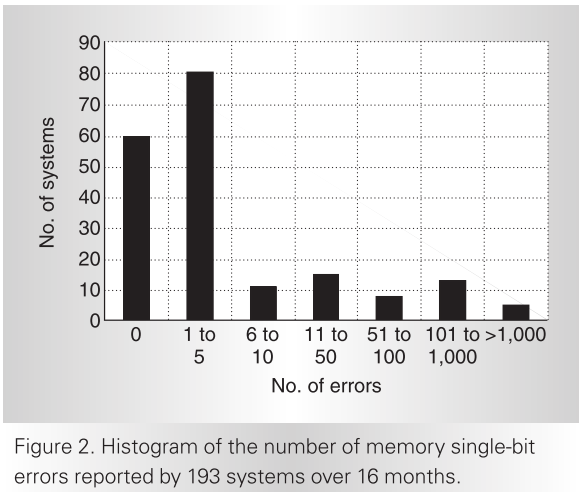
\includegraphics[height=0.35\textheight]{images/Soft-Errors-Histogram.png}
	\mycaption[Histogram of soft error count on 193 data centers over 6 months, taken from \cite{constantinescu2003trends}.]{Histogram taken from \cite{constantinescu2003trends}}
	\label{fig:Soft-Error-Histogram}
\end{figure}

%=======================================================================================================
\section{Causes and Consequences of Soft Errors}
\label{sec:CausesAndConsequencesSoftErrors}
Among the most commonly mentioned causes for soft errors are energetic-particle strikes and fluctuating power supply \cite{kuvaiskii2016haft} \cite{reis2005swift} \cite{zhang2012daft}. Smaller transistor's sizes and lower power voltages allow faster and less energy consuming chips, but it also makes them more susceptible to neutron and alpha particles \cite{constantinescu2003trends}. There have been other studies such as the one in \cite{bautista2016unprotected}, that show evidence that other factors such as temperature and the position of the sun in the sky (actually it would be more correct to say the position of the earth related to the sun) are also related to the presence of soft errors. 

Consequences of soft errors are very different. A single bit flip can be as dangerous to cause a whole system failure or as innocent to provoke absolutely nothing. It is possible to classify the consequences in two types: visible and silent. In first one, there are events such as segmentation faults, which can happen if a bit flips changes the address of a read/store to non accessible memory. Another example of this category is an infinite loop, a bit flip can modify a loop variable resulting in an endless scenario. This type of consequences result in a system detectable event, usually the operating system will notice it and do something about it, like killing the process. Although it is quite serious that the application is stopped and has to be restarted, at least the user knows that something went wrong. 

The other type of consequences are the ones that can be more dangerous, the silent ones. A soft error can go undetected for several reasons. It may be because it happened on an address that was not being used, or that was not going to be used anymore; in either case it does not cause a failure and the system can finish correctly. There are also cases in which depending on the algorithm properties the bit flip can be masked. An iterative process that converges to a result may take a couple of extra iterations because a soft error modified the value being calculated, but can still complete normally; of course, that depends on how the soft error corrupted the value.

But sometimes, in the most unfortunate scenario, the error can alter important data without being detected. The algorithm continues as if nothing happened and the final result can be significantly compromised. In the case of supercomputers that are used for expensive calculations, all the time the system took to finish might have been totally in vain because of a soft error. On certain occasions, the output can be determined to be correct if it falls in a certain interval, depending on the algorithm properties. However, there might be a very unlucky scenario, in which the final value is assumed to be correct and important decisions are made with it.  But, whether or not it can be established that the final value is error-free, all the time spent producing it was wasted; which at the end results in money looses. 

%=======================================================================================================
\section{Detecting Soft Errors}
\label{sec:detectingSoftErrors}

In order to deal with soft errors, two main phases have to be performed: detection and correction. Both of them are important. The first one is usually accomplished through replication, in which the application's instructions are (at least) duplicated and periodical checks are added to discover errors. If the same calculation is done twice, both times the same value should be obtained, if not then it is assumed that a soft error has happened. 

The core idea of replication lies in the low probability of soft errors. Since it is quite unlikely that a bit flip happens even once, by replicating the same instruction and comparing the results, the probability of a soft error corrupting data can be further reduced. What would be the probability of two bit flips happening one right after the other one, in the two precise locations where the results to be compare are, at the same precise bit in both values? It is very much unlikely that this would happen. 

As mentioned in Chapter \ref{chap:intro}, replication can be classified into hardware and software approaches. In the next two subsections each one of them is explained. 

\subsection{Hardware Replication}
\label{subsec:hardwareReplication}

Hardware redundant approaches are transparent to the programmers. Specialized hardware is in charge of replicating and comparing the instructions in order to be reliable against soft errors. Many approaches are mentioned in \cite{reis2005swift} like a \textit{watchdog} processor to compare the values against the main running processor. There are real system like the ones in the Boeing 777 airplanes \cite{yeh1996triple} which replicates the processor and use checkers to validate the redundant computations.

There are other, unusual, ways to perform this phase as well. Upasani \textit{et al} in \cite{upasani2014avoiding} present a physical way to detect particle strikes. The basic idea is to add to the processor \textit{acoustic wave detectors} in order to be able to literally hear a particle strike. A more detailed explanation presented in the same paper: 

``\emph{Alpha and neutron particles can cause soft errors in semiconductor devices. Upon a collision of a particle with a silicon nucleus, the ionization process creates a large number of electron-hole pairs, which subsequently produce phonons and photons. Generation of phonons and photons indicate that a particle strike results into a shockwave of sound, a flash of light or a small amount of heat for a very small period of time. Therefore, we may try to detect particle strikes by detecting the sound, light or heat.}''

The authors in \cite{upasani2014avoiding} choose an acoustic wave detector to identify particles strikes through the sound they generate. They claim that the type of device they propose leads to few false positives and that it is not too costly to be integrated into a common processor. While it is very interesting to know there are other ways to prevent soft errors, such approaches are out of the scope of the current work. 

These specialized hardware are more costly than the commercial ones. Which is to be expected since there are more physical parts and more logic is necessary in the chip. Also, this kind of hardware might not be all the time necessary and if it cannot be turned off, it means such expensive resources may be wasted sometimes. For that, physical replication is not the common choice and although there are many design proposals regarding how is best to replicate in hardware, the current focus of the thesis is software replication used to detect soft errors. 

\subsection{Software Replication}
\label{subsec:softwareReplication}

Software replication approaches are more attractive because, contrary to their counterpart, are much cheaper since they do not require expensive specialized hardware. Of course there are some disadvantages of software-only schemes. They usually incur non negligible resource overhead (time, cores, memory) and they are also not transparent for the programmer. Software redundancy can be distributed into two groups: the first one is thread-local or Instruction Level Redundancy (ILR) error detection and the second one is Redundant Multi-Threading (RMT). 

\subsubsection{Instruction Level Redundancy}
\label{subsec:ILR}

In this category, also called thread-local error detection, all is accomplished in the main thread. Instructions are replicated, creating a separate (shadow) data flow along the original one, and integrity checks are added in order to detect errors. The second data flow works using different registers, therefore allowing safe value comparisons by the checks. Also, since there is no dependency between the master and shadow instructions they can potentially be executed in parallel leveraging from instruction-level-parallelism present in modern processors; the next two examples of code show a common ILR code transformation \cite{kuvaiskii2016haft}. 

\begin{flushleft}
\underline{Original Code}
\end{flushleft}

\begin{lstlisting}[language = pseudocode]
a = 5
b = 8
c = a + b
print(c)
\end{lstlisting}

\begin{flushleft}
\underline{Replicated code with ILR}
\end{flushleft}
\begin{lstlisting}[language = pseudocode]
a1 = 5
b1 = 8
a2 = 5
b2 = 8
c1 = a1 + b1
c2 = a2 + b2
check c1, c2
print(c)
\end{lstlisting}

\subsubsection{Redundant Multi-Threading}
\label{subsec:BacgroundRedundantMultiThreading}

The second group of software replication is redundant multi-threading error detection. Here, two threads distribute the work, they can be called \textit{producer} or \textit{leading} thread and \textit{consumer} or \textit{trailing} thread. Redundant multi-threading has some advantages over thread-local error detection. In the latter, the code size of the application increases significantly and all the checks are added on the critical path of the program, resulting in a lot of performance overhead. Redundant multi-threading tries to solve this issue by distributing the work in two threads; this makes sense since multi-core chips are so popular in the market \cite{mitropoulou2016comet}. 

Redundant multi-threading (RMT) \cite{mitropoulou2016comet} \cite{wang2007compiler} \cite{zhang2012daft} tries to reduce the performance overhead added in ILR soft error detection by using two threads. The original application code is replicated in both threads. Every time a value needs to be checked for soft errors, the leading thread produces the value, the trailing thread consumes it and checks it against its own calculated value. RMT removes the checks from the critical path of the application by having the second thread be the one that compares the results. Figures \ref{fig:CodeTransformationWithRMT} and \ref{fig:CodeTransformationWithRMTCyclic} show examples of code transformation using a RMT approach, where the original code is duplicated in the leading and trailing thread; \textbf{boldface} is used to denote the new instructions added for thread communication, both Figures resemble the way authors from an approach called DAFT \cite{zhang2012daft} explain different communications patterns between the threads.

One downside of redundant multi-threading is that the threads need to be in constant communication, in order to be able to compare the results each of them obtained. Therefore, the inter-thread data sharing mechanism is the performance bottleneck of such solutions. This problem does not happen in the thread-local variant since everything happens in the same thread. Still, there are are some options such as \cite{mitropoulou2016comet} \cite{wang2007compiler} \cite{zhang2012daft} that are able to obtain acceptable performance overheads. In the current thesis we focus on redundant multi-threading approaches.

\begin{figure}[h]
	\centering
	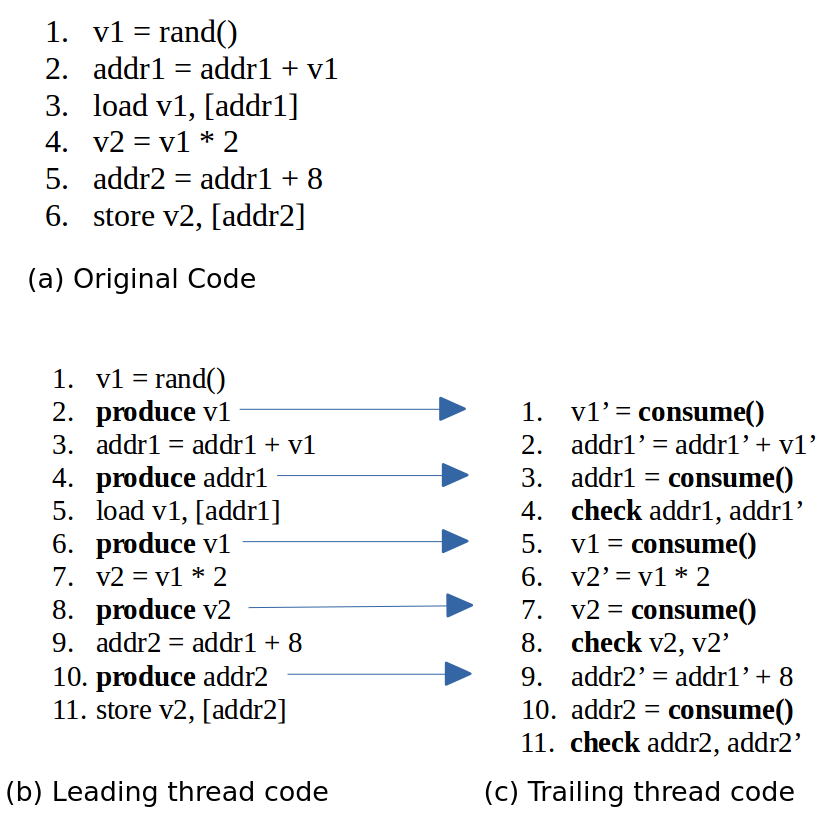
\includegraphics[height=0.5\textheight]{images/CodeTransformation.png}
	\mycaption[Asynchronous Code Transformation using RMT]{Asynchronous Code Transformation using RMT}
	\label{fig:CodeTransformationWithRMT}
\end{figure}

There are important facts about Figure \ref{fig:CodeTransformationWithRMT}, specially regarding which original instructions are duplicated. It is common practice \cite{mitropoulou2016comet} \cite{wang2007compiler} \cite{zhang2012daft} that library function calls as well as store/loads to/from memory are excluded from replication. In the case of library functions, since the code is not available to instrument and the result from two calls of the same method might be different (as with the case of ``\textit{rand()}'' that generates random numbers), the returned value of the procedure is shared from the leading to the trailing thread. An example is shown with instruction 1 from Figure \ref{fig:CodeTransformationWithRMT}.a, that generates instruction 2 in Figure \ref{fig:CodeTransformationWithRMT}.b and instruction 1 in Figure \ref{fig:CodeTransformationWithRMT}.c. 

Stores and loads from memory are also not replicated but, the addresses and values are checked in the trailing thread in order to make sure those operations run free of error. The reason is because soft error detection techniques focus on faults happening in the processor and not in the memory, since ECC and other protection mechanisms exist for RAM, but the processor's registers are still vulnerable. That is why, once a value has been loaded from memory, it is then shared from the leading to the trailing thread; such as instruction 3 in Figure \ref{fig:CodeTransformationWithRMT}.a that produces instructions 6 and 5 in Figures \ref{fig:CodeTransformationWithRMT}.b and \ref{fig:CodeTransformationWithRMT}.c, respectively. 

\begin{flushleft}
\underline{Asynchronous Communication Pattern}
\end{flushleft}

Inter-thread communication is commonly done via a Singe Producer/Single Consumer (SPSC) queue. DAFT \cite{zhang2012daft} categorizes some communications patterns among Redundant Multi-Threading approaches. In the example of Figure \ref{fig:CodeTransformationWithRMT} there is an asynchronous (also called unidirectional) communication pattern, where the producer does not wait for the check of the consumer, it simply pushes a value into the queue and keeps on running. In this case, if an error occurs in the leading thread that causes data corruption, the trailing thread will detect it later. But since the producer may have already made other operations with an incorrect value, the whole process must be stopped or fixed. As long as the instructions the leading thread performs do not escape its scope (local thread memory), this mechanism works fine. 

The use of \textit{volatile variable accesses} makes the problem more complicated. A volatile variable is one that may be modified in ways unknown to the implementation or have other unknown side effects. Memory-mapped IO accesses are an example of volatile variable accesses \cite{zhang2012daft}, like printing to the monitor, writing to a file, communicating through the network. Therefore, if the leading thread executes one of these operations with a soft error, the consequences can be catastrophic and irreversible; corrupting a file or sending incorrect data to another node are some examples. Therefore, it would not make sense that the trailing thread reports that an error has occurred, after it has already provoked a terrible irremediable effect. However, there might be cases where there are no volatile stores and this communication pattern is sufficient.

\begin{flushleft}
\underline{Synchronous Communication Pattern}
\end{flushleft}

On the other hand, when there are volatile stores the above mentioned scheme is not safe enough. Because of such problem, the safest option is that every time the leading thread performs any memory operation, instead of continuing, it waits for the trailing check to confirm that such operation is error-free and then makes forward progress. So, the communication pattern would be synchronous (or bi-directional). An example of this approach is shown is Figure \ref{fig:CodeTransformationWithRMTCyclic}; the right-to-left arrows denote the times the producer has to wait for the consumer. Sadly, the downside of such approach, is that it increases the already non negligible overhead of asynchronous inter-thread communication, as demonstrated in DAFT \cite{zhang2012daft}. The producer now spends a lot of time waiting for the consumer, rather than actually doing something useful. 

\begin{figure}[h]
	\centering
	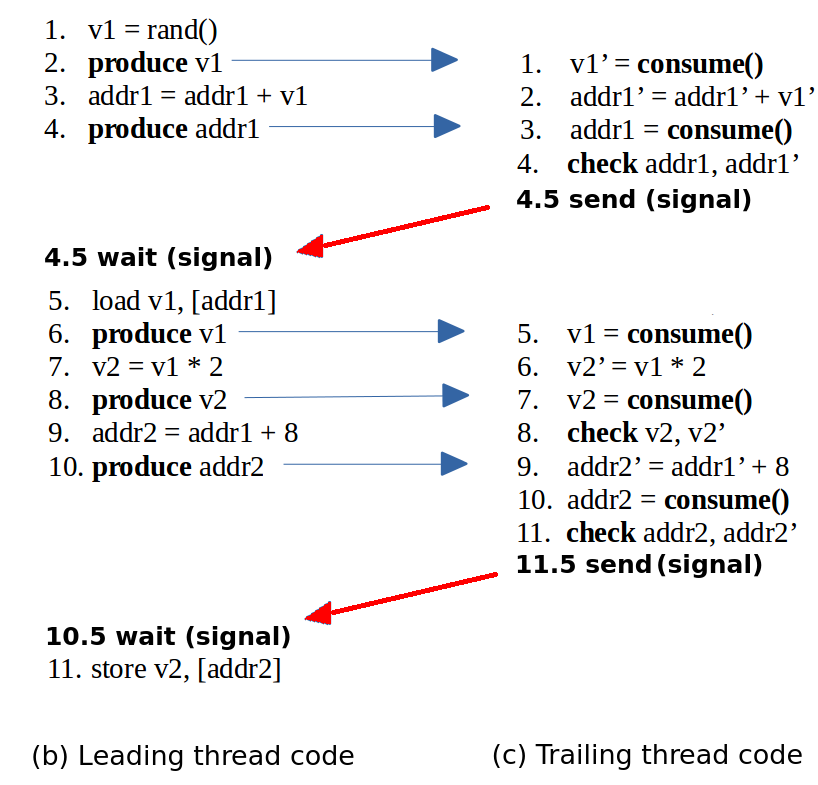
\includegraphics[height=0.5\textheight]{images/CodeTransformation-Cyclic.png}
	\mycaption[Synchronous Communication Pattern in RMT]{Synchronous Communication Pattern in RMT}
	\label{fig:CodeTransformationWithRMTCyclic}
\end{figure}

\pagebreak

\begin{flushleft}
\underline{Semi-Synchronous Communication Pattern}
\end{flushleft}

There is a third option in between waiting for the result of the trailing thread on every single memory access or just let the producer make forward process without any synchronization whatsoever, we called it \textit{semi-synchronous communication pattern}. The basic idea is to make sure that only volatile variable accesses are correct before performing them. This is done in the literature by either synchronizing with the consumer only for those cases, or adding comparisons in the leading thread (an ILR approach) \cite{wang2007compiler} \cite{zhang2012daft}. Figure \ref{fig:SemiSyncRMT} shows an example of this scheme the way \cite{wang2007compiler} doest it. 

\begin{figure}[H]
	\centering
	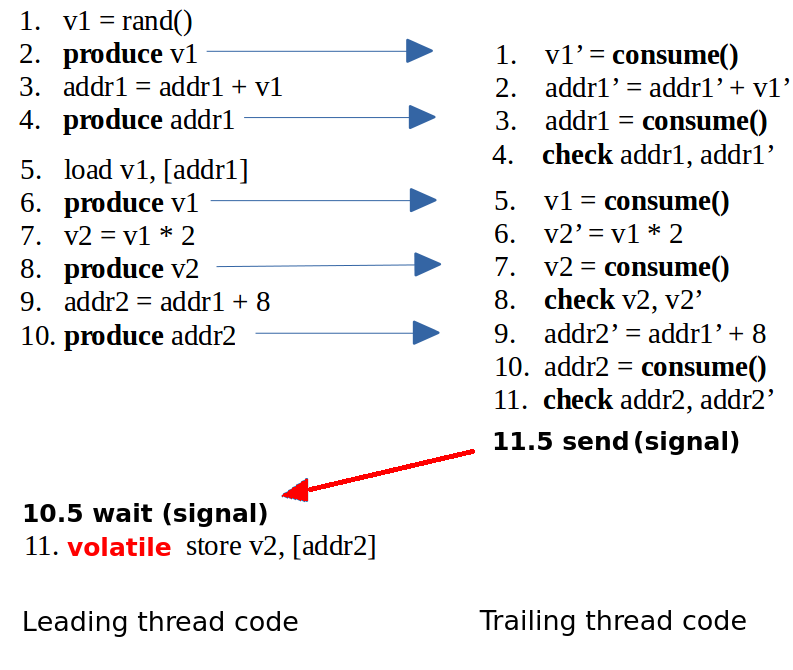
\includegraphics[scale=0.5]{images/Semi-Sync-Communication.png}
	\mycaption[Semi-Synchronous Communication Pattern in RMT]{Semi-Synchronous Communication Pattern in RMT}
	\label{fig:SemiSyncRMT}
\end{figure}

Such scheme reduces the inter-thread communication cost but, poses other troubles. One problem is to be able to determine volatile variable accesses and their dependencies. Such information might be available at compile time or it might be more difficult to obtain, like functions accessed by pointers. If ILR is chosen to protect volatile accesses, then the dependencies of the stores must be also replicated in the leading thread. In the case where a simple variable, already corrupted due to a soft error, is used to obtain the memory address of the volatile store, it does not help to duplicate the calculation of the memory address. Every data dependency has to be verified before performing the store. So, there might be cases where the leading thread actually ends up replicating everything because of data dependencies, which will defeat the purpose of redundant multi-threading. 

Another problem with such scheme is that since the producer thread is able to run in some cases without the check of the consumer, it might trigger exceptions. A division by zero or segmentation fault can occur because of a change in a value or an address. Such problems should not happen in a soft-error-free scenario so there might not be appropriate handlers for them in the original code; which will usually cause the program to be killed by the OS. One option, if one needs to provide recovery from this scene, is to add artificial handlers. Furthermore, they should be able to determine if the exception was due to natural causes, in which case the error should be passed to the application's original handlers (if any); or if it was due a soft error, where it should be managed differently. Another strategy could be to have the application be executed by an external program, one that can monitor and make decisions in cases where the original executable is unable to recuperate itself \cite{wang2007compiler} \cite{zhang2012daft}. Figure \ref{fig:RMT} shows an overview of the different communication patterns in Redundant Multi-Threading approaches. 

\begin{figure}[H]
	\centering
	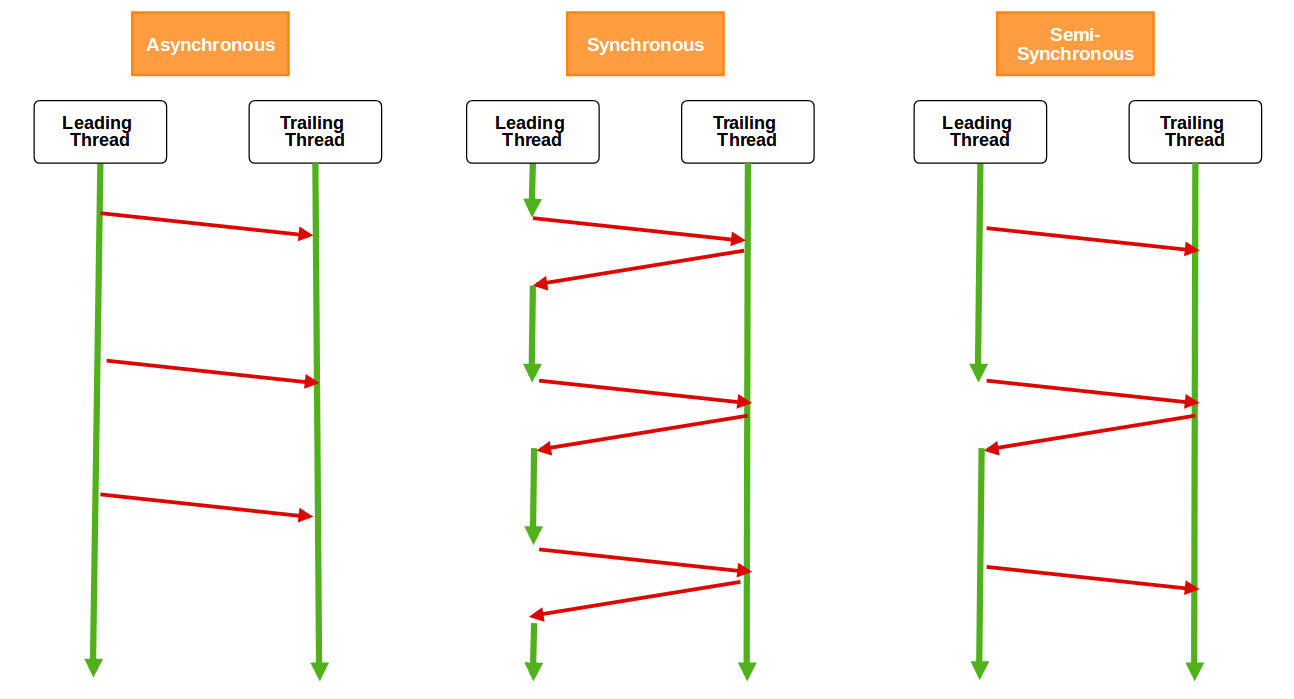
\includegraphics[scale=0.36]{images/RMT.png}
	\mycaption[RMT Communication Patterns]{Redundant Multi-Threading Communication Patterns}
	\label{fig:RMT}
\end{figure}

\pagebreak

%=======================================================================================================
\section{Correcting Soft Errors}
\label{sec:correctionPhase}

\begin{wrapfigure}{r}{7.5cm}	
	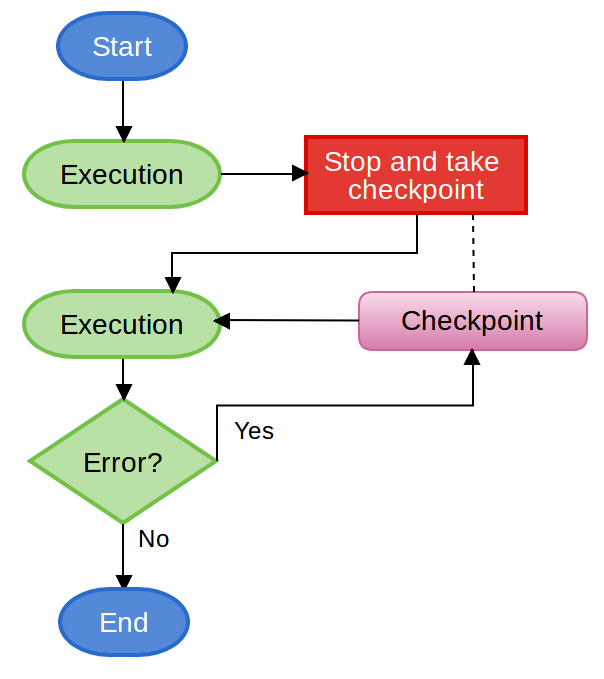
\includegraphics[width=7.5cm]{images/Checkpointing.png}
	\mycaption[Checkpointing Diagram]{Checkpointing Diagram}
    \label{fig:Checkpointing}
\end{wrapfigure}

The correction phase is the one that executes only when a soft error has been identified. Checkpointing approaches can be used in the correction phase, like mentioned in \cite{calhoun2017towards} \cite{kuvaiskii2016haft} \cite{mitropoulou2016comet}. Figure \ref{fig:Checkpointing} shows the diagram of this technique. Every certain amount of time, or instructions, the application's state (a checkpoint) is saved somewhere. The information saved should be enough so the program can restart the execution based on it. The state usually means the values of the variables at certain point in time and it is very important to make sure that every saved data is error-free. Checkpointing comes with a performance overhead, there is a penalty every time the application must be stopped in order to collect its state; depending on how much is saved each time and how many times a checkpoint is taken, the overhead varies. The benefit of checkpointing is that if an error is detected, the program is restored to the latest safe point and (hopefully) not the beginning of the execution. Since a transient fault is something very unlikely, the cost of recuperating the system in case of error is not typically a problem, but the cost of maintaining the checkpoints is what negatively impacts performance.  

Another option to recover from soft errors is having Triple Modular Redundancy (TMR). Figure \ref{fig:TripleModularRedundancy} shows the diagram of such technique. Two extra copies of the calculation are performed and a majority vote is used each time to decide the correct result. There is no explicit correction phase in this approach because, a soft error would be detected by having one of the three copies being different than the rest (assuming of course a Single Event Upset, SEU). And the correction phase, would be having the copy that diverges from the other two discarded and letting the program continue from there on with the other two; or the failed copy can be restored to the state of the other two. Note that this scheme has both identification and correction of soft errors, however TMR in general is a very expensive approach since it maintains two extra copies of the application \cite{calhoun2017towards}. 

\begin{figure}[h]
	\centering
	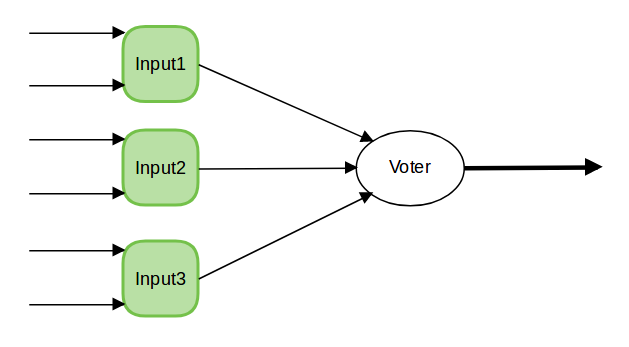
\includegraphics[scale=0.5]{images/TripleModularRedundancy.png}
	\mycaption[Triple Modular Redundancy Diagram]{Triple Modular Redundancy Diagram}
	\label{fig:TripleModularRedundancy}
\end{figure}

These techniques have been already studied for a while and are a popular choice to correct soft errors \cite{kuvaiskii2016haft} \cite{kuvaiskii2016elzar}. It is also not uncommon to provide only soft error detection solutions, since error correction methods can be later included \cite{mitropoulou2016comet} \cite{wang2007compiler} \cite{zhang2012daft}. No matter how the execution should be restored, if needed, the replication phase that allows error detection should be done efficiently. Because of these reasons, the thesis focus on soft error detection, specifically a redundant multi-threading approach. 

%=======================================================================================================
%\section{Current Multi-core chip features}
%\label{sec:multi-core-features}

%Current multi-core processors features like Hardware Transactional Memory and Hyper-Threading may help reduce the overall overhead when dealing with soft errors. 

%\subsection{Hardware Transactional Memory}
%\label{subsec:HTM} 
%Transactional Memory (TM) follows the same principles as database transactions, where a set of instructions (a transaction) are managed as if they were just one instruction. If the transaction succeeds then all operations are atomically committed to the database. If not, every operation is reverted and the state of the database remains the same as when the transaction began. One difference with TM is that the goal of a transaction is not to commit changes to a database but to the main memory of a processor, as shown in Figure \ref{fig:Transactional-Memory}. For that when a transaction begins, the values of modified variables are stored in the cache of the core and if no \textit{collisions} are detected then those changes are atomically committed to RAM, so every other core can view these new results. A collision usually means a memory conflict among concurrent transactions, such as write-write/read-write conflicts; a transaction reads or writes the same address that another simultaneous transaction has already modified \cite{herlihy1993transactional}.

%\begin{figure}[h]
%	\centering
%	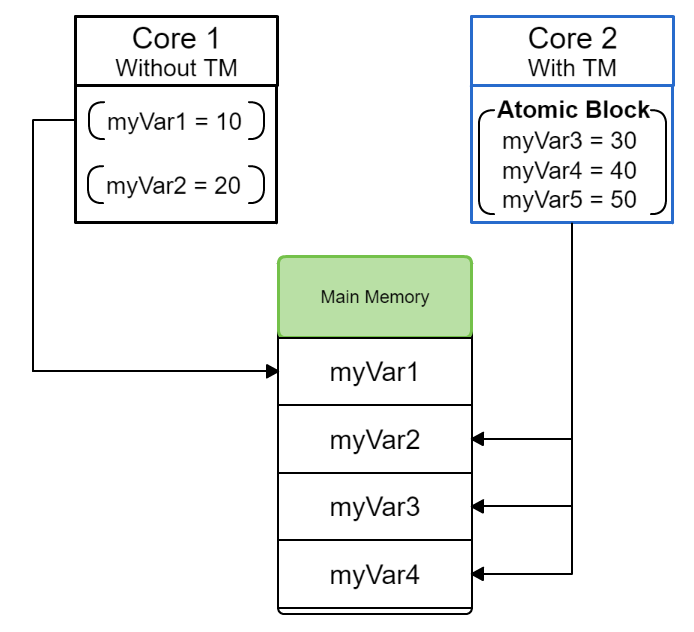
\includegraphics[height=0.35\textheight]{images/TM.png}
%	\mycaption[Atomic block execution with Transactional Memory]{Atomic block execution with Transactional Memory}
%	\label{fig:Transactional-Memory}
%\end{figure}

%There are software and hardware implementations of Transactional Memory. As it is expected from sort of comparisons, software options are usually more flexible but the hardware option has better performance. EXPAND THIS, LOOK FOR MORE REFERENCES, NOT SURE WE WANT TO EXPAND THIS... MAYBE IT WILL BE DELETED 

%Transactional Synchronization Extensions (TSX) is the Intel version of Hardware Transactional Memory and was proposed as part of the Haswell Instruction set architecture \cite{hammarlund2014haswell}. This document focus on multi-processors chips that have this feature, specifically on the Intel Restricted Transactional Memory (RTM) interface, which exposes a new set of primitives: 

%\begin{itemize}
%	\item \textit{\_xbegin}, initializes a new transaction.
%	\item \textit{\_xend}, marks the current transaction as successful, and therefore commits atomically the changes to RAM. 
%	\item \textit{\_xtest}, tells if one is inside a transaction.
%	\item \textit{\_xabort}, explicitly causes an abortion of the current transaction and restores the state of the core as it was at the latest successful execution of \textit{\_xbegin}.
%\end{itemize}

%Transactional Memory was originally proposed as a better way to achieve high performance mutual exclusion, yet easy to implement, in applications with concurrent access to shared memory. Intel TSX ensures the same results as having a coarse-grained lock, but allows non conflictive operations to occur without the delay that coarse grained locks would have injected \cite{Coarse-grained-TSX}. 

%Internally in Intel TSX, transactions have a read and write sets, to keep track of what has been consulted and modified, such information is temporarily stored in the L1 cache. The execution model is optimistic, meaning it does not block all the time (as a mutex does) a concurrent execution of the code. Instead, to detect conflicts in parallel transactions an optimized cache coherency protocol is used; having two transaction with the same memory location in their read sets does not cause an abortion, but if one reads a variable that is also present in another transaction's write set, at least one transaction aborts. If such thing happens (explicitly or implicitly) the execution jumps to an abort handler (that has to be provided), where usually the transaction is retried a number of times before going to a fallback path where progress should be guaranteed, in case the code cannot be executed transactionally \cite{kuvaiskii2016haft}.

% PERHAPS MOVE THIS TO CHAPTER 3, we hare presenting the feature here, it is not the place to discuss about downsides --- Even though it is not its original purpose, Intel TSX also provides strong isolation guarantees and a way to rollback that can be utilized as a recovery mechanism. But, there are several design choices that limit the use of this feature for fault tolerance. First of all, Intel does not guarantee that a transaction will eventually commit, even when applied to sequential code \cite{yoo2013performance}. Since it uses the core's cache to temporarily keep track of reads and writes, the amount of memory is limited to the physical capabilities of the processor. Also there is a time limit (based on the interval of timer interrupts) of how much a transaction can last before it is aborted \cite{kuvaiskii2016haft}. Lastly there are ``unsafe'' operations (such as system calls) that force a core to abort any active transactions \cite{kuvaiskii2016haft}. Thus, the importance of a fallback path is vital. 

\section{Simultaneous Multi-Threading}
\label{sec:simultaneousMultiThreading}
\textit{Superscalar} microprocessors implement a form of parallelism called \textit{instruction-level-parallelism}, which allows them to execute more than one instruction during a clock cycle. It is done by concurrently dispatching several instructions to different executions units of the processor. \textit{Simultaneous Multi-Threading} (SMT) is a technique to increase the performance of a superscalar microprocessor. It allows independent threads to better utilize the physical resources of a processor. A machine with SMT capabilities tries to allow multiple threads to execute simultaneously in the same cycle, on different functional units \cite{reinhardt2000detectionSimultaneousMultithreading}. 

\subsection{Intel Hyper-Threading}
\label{subsec:hyper-treading}
Intel's \textit{Hyper-Threading} Technology brings the concept of simultaneous multi-threading to the Intel Architecture. Hyper-Threading makes a single physical processor appear as (at least) two logical processors. The physical execution resources are shared and the \textit{architecture state} is duplicated for the logical processors. Each logical processor has its complete architecture state which consists of registers. Among them are the general purpose registers, the advanced programmable interrupt controller (APIC) registers, the control registers and some machine state registers; Figure \ref{fig:Hyper-Threading} shows how a core with Hyper-Threading technology looks like. From a software perspective, since there are multiple architecture states, the one physical processor appears to be as multiple processors. This means operating systems and user programs can schedule processes or threads to logical processors as they would on multiple physical processors. From a micro-architecture perspective, this means that instructions from both logical processors will persist and execute simultaneously on shared execution resources \cite{Hyper-Threading}.

\begin{figure}[h]
	\centering
	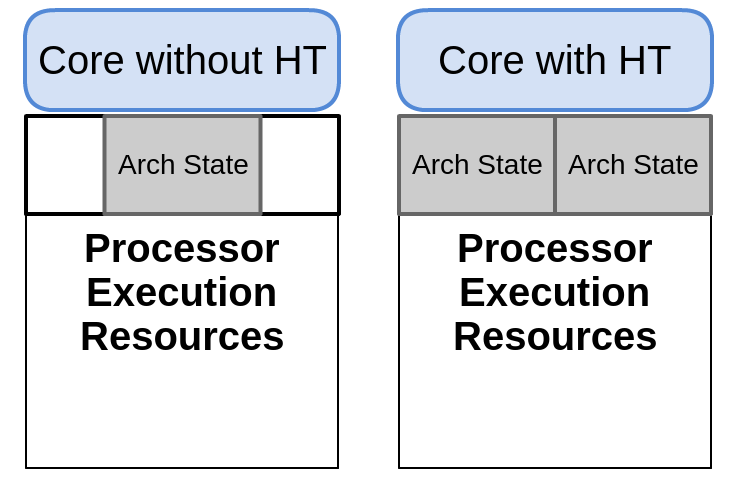
\includegraphics[height=0.35\textheight]{images/Hyper-Threading.png}
	\mycaption[Core without and with Hyper-Threading]{Core without and with Hyper-Threading}
	\label{fig:Hyper-Threading}
\end{figure}

Intel in \cite{Hyper-Threading} claims that the number of transistors necessary to store another architecture state is an extremely small fraction of the total. But doing so favors a much more efficient resource usage, which translates to greater performance at very low cost. The logical processors nearly share all other physical resources, such as caches, execution units, control logic, branch predictors and buses. 

Hyper-Threading does not do much for single thread workloads, but when multiple threads can run in parallel there may be a significant performance improvement, because it ensures that when one logical processor is stalled, the other logical processing unit (on the same core) can continue to make forward  progress (without context switching). A logical processor may be temporarily stalled for a variety of reasons, including servicing cache misses, handling  branch mispredictions, or waiting for the results of a previous instruction \cite{Hyper-Threading}.

Although Intel claims that common server applications can benefit from hyper-threading, obtaining around 30\% of performance improvement \cite{Hyper-Threading}, there are cases when Hyper-Threading does not yield an improvement or even worse represents an overhead, as analyzed in \cite{saini2011impact}. Memory bound applications, in which the bottleneck is the memory latency, can benefit from Hyper-Threading. While one hyper-thread is waiting for a memory access, the other one can utilize the execution units, leading to a better resource usage. On the other hand, for CPU-intensive programs that tend to keep the execution units busy, having to share such resources with another thread will not represent an enhancement. 

The use of hyper-threading in the detection phase of soft errors can be of a lot of help. Since in redundant multi-threading approaches the bottleneck is inter-thread communication, the fact that hyper-threads share the L1 level cache can be exploited. Instead of having to send data from one core to another, usually through the last level of cache (or even worse, through main memory), exchanging values using L1 cache can benefit performance significantly. Figure \ref{fig:ProcessorWithHT} exemplifies this situation.  

\begin{figure}[H]
	\centering
	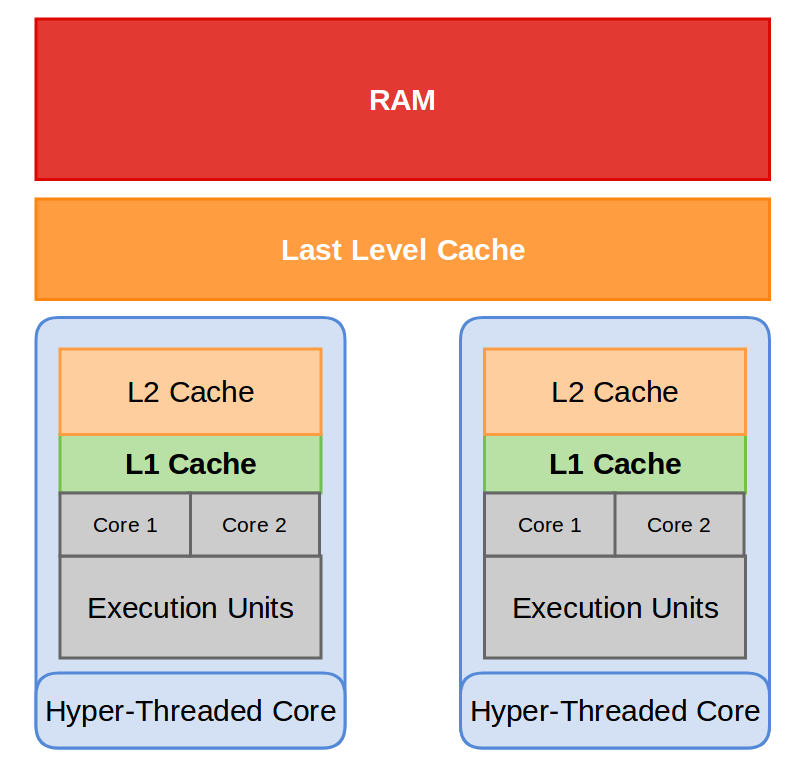
\includegraphics[scale=0.5]{images/HTProcessor.png}
	\mycaption[Diagram of Hyper-Threaded Processor]{Diagram of Hyper-Threaded Processor}
	\label{fig:ProcessorWithHT}
\end{figure}





